
%
%  $Description: Author guidelines and sample document in LaTeX 2.09$ 
%
%  $Author: ienne $
%  $Date: 1995/09/15 15:20:59 $
%  $Revision: 1.4 $
%

\documentclass[times, 10pt,twocolumn]{article} 
\usepackage{paper}
\usepackage{times}
\usepackage{graphicx}
\usepackage{float}
\usepackage{amsmath}

%\documentstyle[times,art10,twocolumn,latex8]{article}

%------------------------------------------------------------------------- 
% take the % away on next line to produce the final camera-ready version 
\pagestyle{empty}

%------------------------------------------------------------------------- 
\begin{document}

\title{Citi Bike Usage Balancing through Congestion Pricing}

\author{Paul Griffioen\\Dept. of Electrical and Computer Engineering\\Carnegie Mellon University\\ pgriffi1@andrew.cmu.edu\\
% For a paper whose authors are all at the same institution, 
% omit the following lines up until the closing ``}''.
% Additional authors and addresses can be added with ``\and'', 
% just like the second author.
\and
Anthony Jin\\Dept. of Electrical and Computer Engineering\\Carnegie Mellon University\\xiaoxiaj@andrew.cmu.edu\\
}

\maketitle
\thispagestyle{empty}

%------------------------------------------------------------------------- 
\section{Abstract}

The issue of congestion in bicycle sharing systems is prevalent in many cities. This project proposes an incentive-based pricing scheme for New York City's Citi Bike system that minimizes bicycle congestion. It approaches bicycle sharing systems from a network perspective, analyzing and optimizing the network by providing monetary incentives to users with the intent of modifying network properties. These monetary incentives are the output of a much larger optimization problem designed to minimize poor service quality. To demonstrate the effectiveness of this approach, the Citi Bike system is modeled and simulated using MATLAB, where monetary incentives are given to users such that poor service quality is minimized.

%------------------------------------------------------------------------- 
\section{Introduction and Motivation}

The Citi Bike system, located in New York City, is one of many bicycle sharing systems that exist in the world. Since users unlock a bike at one station and drop it off at another station, bikes tend to follow unidirectional flows at various times of the day. As a result, some stations have few to no bikes at them while others are completely full.

This unidirectional flow of bikes frustrates users who would like to pick up a bike from an empty station or drop off a bike at a full station. As a result, this project seeks to address the issue of system congestion through a pricing scheme based on the optimization of network structure and dynamics. Looking at the problem from a network perspective is a unique approach that has not been considered with previous work. In the end, this project seeks to analyze the Citi Bike network and minimize poor service quality by modifying its structure through changing people's incentives.

%------------------------------------------------------------------------- 
\section{Previous Work}

Previous work has taken many viewpoints to solve the bike sharing congestion problem. The work in \cite{incentives} proposes a dynamic incentives system that involves future traffic prediction, truck-based re-positioning policies, and schema to compute monetary incentives for users. The authors in \cite{redistribution} use a similar approach, combining staff-based dynamic vehicle distribution and real-time pricing incentives for customers. In contrast, \cite{management} and \cite{redistribution} look at the inventory management of individual bike-sharing stations and formulate appropriate convex optimization problems. Similar to the aforementioned approaches, this project will address the congestion problem as a convex optimization problem and introduce a congestion-based pricing scheme to modify user incentives. Unlike prior work, however, it takes a network standpoint and models the Citi Bike system as a dynamic network.

%------------------------------------------------------------------------- 
\section{Approach}

The Citi Bike network is built using available data from Citi Bike's website \cite{dataset}. The nodes represent different bike stations and the weighted links represent the number of trips made from one station to another in a certain time period $t$. A few node and edge attributes are also of interest. Each node (bike station) has an identification number, latitude and longitude, maximum capacity, and current number of stored bikes. Meanwhile, each edge (bike trip) has a bike identification number and a user age. These attributes are used as inputs in the convex optimization problem for the incentive-based pricing scheme.

The trip data in \cite{dataset} does not include explicit information about the addition or removal of bikes to the system or the transfer of bikes by truck from one station to another. Consequently, this project can only analyze bike trips from one station to another. In addition, there is no information about the number of bikes at particular stations at specific points in time. As a result, an initialization procedure is used to infer this information.

\subsection{Initialization Procedure}
The objective of the initialization procedure is to determine an initial state of the Citi Bike system at any point in time. The procedure begins by identifying a start time and assuming that no bikes are initially in the system. Over a specified time period, bikes are added to the system using incoming trip data for each station and are tracked by their identification numbers to determine which stations they are at. At the end of this period, it is assumed that all bikes have been added to the system, and each station is assigned with an initial number of bikes. Future trip data can now be used to determine the number of bikes at particular stations at any time after the initialization procedure.

\subsection{Convex Optimization Overview}

A convex optimization problem, used to compute monetary incentives for users, is formulated such that poor service quality is minimized subject to budget constraints. This convex optimization problem computes the payment for a user after a pair of alternative stations for the user has already been determined. As a result, the convex optimization problem is solved locally on a trip-by-trip basis rather than globally to assign a set of payments to a set of users. The reason the first approach is taken is because it can be implemented in real life. The other approach is unrealistic because it assumes all bike trips within a specified time period occur instantaneously. Since this approach cannot be implemented in real life, we first compute a pair of alternative stations and then use convex optimization to map an appropriate payment to that pair of alternative stations. Consequently, this approach decongests the Citi Bike network from a local perspective. A few functions and parameters on which the convex optimization problem depends are defined in the next section.

\subsection{Function and Parameter Definitions}

We consulted \cite{incentives} in order to accurately define a function that models the maximum distance a user is willing to walk to a pair of alternative stations. The authors in \cite{incentives} conducted a survey of users for a real-world bike sharing system in a European city to elicit user preferences about additional distances they are willing walk. While roughly 20\% of the responses were "unwilling to walk" or "unwilling to participate at any cost," most of the other participants were only willing to walk less than or equal to one mile. Additionally, the results of the survey suggest that the relationship between the cumulative distribution of willingness to walk and the maximum walking distance is a decaying exponential (namely, more people are willing to walk a shorter additional distance than a longer one).

We speculate that there is a direct correlation between a user's age and his or her willingness to walk an additional distance. In other words, when given the same incentives, the additional distance an elderly person is willing to walk is less than that of a young person. As a result, we define a function that computes the maximum distance a user is willing to walk as a function of the user's age. In this function, $u = \{u_1, u_2, ..., u_n\}$ represents the set of $n$ users in the Citi Bike network during time interval $t$, $A_u$ represents the age of user $u$, and $r_u$ represents the maximum distance user $u$ is willing to walk. $r_u$ is modeled as a decaying exponential function of $A_u$ ranging from $r_u^{min} = 0.1$ to $r_u^{max} = 1$, where the units of $r_u$ are miles. If a user is more than 60 years old, he or she is automatically assigned with $r_u^{min}$. Similarly, a user younger than 18 years old is assigned with $r_u^{max}$. In summary, $r_u$ is expressed as
\begin{equation}
%r_u = f(A_u)
%r_u = 2.683e^{-0.055A_u}
r_u = \left\{
        \begin{array}{lll}
            1 & \quad 0 \leq A_u \leq 18 \\
            2.683e^{-0.055A_u} & \quad 18 \leq A_u \leq 60 \\
            0.1 & \quad A_u \geq 60 \\
        \end{array}
    \right.
\end{equation}

The distance (in miles) between a pair of stations $s_1$ and $s_2$ is calculated using the Haversine formula in Equation 2, which relies on equations 3-5 to compute its value. Here, $l_{lat1}$, $l_{lat2}$, $l_{lon1}$, and $l_{lon2}$ represent the latitudes and longitudes of the two stations, and the constant 7922 represents the diameter of the earth in miles.
\begin{equation}
dist(s_1,s_2) = 7922\arctan{\frac{\sqrt{a}}{\sqrt{1-a}}}
\end{equation}
\begin{equation}
a = (\sin{\frac{1}{2}d_{lat}})^2+(\cos{l_{lat1}})(\cos{l_{lat2}})(\sin{\frac{1}{2}d_{lon}})^2
\end{equation}
\begin{equation}
d_{lon} = l_{lon2} - l_{lon1}
\end{equation}
\begin{equation}
d_{lat} = l_{lat2} - l_{lat1}
\end{equation}

The set of $m$ bike stations in the network is denoted by $s = \{s_1, s_2, ..., s_m\}$. Each station is associated with a maximum capacity $C_s$ and two congestion levels at any given time. $G_{spu}$ is the station's congestion for a user who wants to pick up a bike, measuring the percentage of open docks at the station. Similarly, $G_{sdu}$ is the station's congestion for a user who wants to drop off a bike, measuring the percentage of stored bikes at the station when the user arrives. As a result, both $G_{spu}$ and $G_{sdu}$ vary between 0 and 1, where 1 represents complete congestion and 0 represents no congestion. In the following equations, $v_s$ denotes the current number of bikes at the station, and $v_{sf}$ represents the number of bikes that are added or subtracted from $v_s$ while the user travels to the drop-off station.
\begin{equation}
G_{spu} = \frac{C_s-v_s}{C_s}
\end{equation}
\begin{equation}
G_{sdu} = \frac{v_s+v_{sf}}{C_s}
\end{equation}

When a user wants to go on a bike trip, $s_{pu}$ and $s_{du}$ represent his or her intended pick-up and drop-off stations, respectively. The following process is used to compute a pair of alternative stations for the user. First, only pick-up and drop-off stations that lie within a radius $r_u$ from $s_{pu}$ and $s_{du}$, respectively, are considered. These candidate pick-up and drop-off stations are denoted by $s_{puc} = \{s_{puc}^1, s_{puc}^2, ..., s_{puc}^i\}$ and $s_{duc} = \{s_{duc}^1, s_{duc}^2, ..., s_{duc}^j\}$, respectively. Second, the total distance between the intended stations and the candidate stations must be no more than $r_u$ since the user is only willing to walk a maximum additional distance $r_u$. Thus, the set of pairs $\{\{s_{puc}^k,s_{duc}^l\}, ...\}$ denotes all combinations of element pairs between $s_{puc}$ and $s_{duc}$ where
\begin{equation}
d_u = dist(s_{puc}^k, s_{pu}) + dist(s_{duc}^l, s_{du}) \leq r_u
\end{equation}
Here, $d_u$ represents the total distance the user would have to walk to use the pair of alternative stations.
%\begin{equation}
%d_{pu} = dist(s_{pu}, s)
%\end{equation}
%\begin{equation}
%d_{du} = dist(s_{du}, s)
%\end{equation}
Lastly, the pair of stations in $\{\{s_{puc}^k,s_{duc}^l\}, ...\}$ with the smallest total congestion (smallest $G_{spu}+G_{sdu}$) is selected as the user's pair of alternative stations.

\subsection{Constraints}
A payment $p_u$ is given to the user if he or she decides to use the pair of alternative stations. However, this payment is subject to a few constraints given in Equation 9, including the fact that $p_u$ cannot be negative. Due to budget constraints, $p_u$ must also be less than the maximum allowable payment. This maximum payment is equal to the total spending budget $B$ for time interval $t$ divided by the number of active users $n$ in the network during time interval $t$.
\begin{equation}
0 \leq p_u \leq \frac{B}{n}
\end{equation}

%$G_s$ represents the congestion level at station $s$, where $C_s$ denotes the maximum capacity at station $s$, $v_s$ denotes the current number of bikes at station $s$, and $o_s$ and $i_s$ denote the out-degree and in-degree of station $s$, respectively. $k$ is a constant that weights the impact of the out-degree and in-degree on the congestion level.
%\begin{equation}
%G_s = \frac{1}{2}C_s - v_s - k(i_s - o_s)
%\end{equation}
%Next, $s_{puc} = \{s_{puc}^1, s_{puc}^2, ...\}$ and $s_{duc} = \{s_{duc}^1, s_{duc}^2, ...\}$ represent user $u$'s set of candidate stations for pick-up and drop-off, respectively. These sets of candidate stations will be determined by the fact that $d_{pu} \leq r_u$ and $d_{du} \leq r_u$. $s_{puc}$ will only contain stations with $G_s \leq 0$, and $s_{duc}$ will only contain stations with $G_s \geq 0$.
%\begin{equation}
%s_{puc} = f(G_s, d_{pu}, r_u)
%\end{equation}
%\begin{equation}
%s_{duc} = f(G_s, d_{du}, r_u)
%\end{equation}
%$d_{puc} = \{d_{puc}^1, d_{puc}^2, ...\}$ and $d_{duc} = \{d_{duc}^1, d_{duc}^2, ...\}$ denote the set of distances between the set of stations $s_{puc}$ and station $s_{pu}$ or between the set of stations $s_{duc}$ and station $s_{du}$, respectively.
%\begin{equation}
%d_{puc} = dist(s_{pu}, s_{puc})
%\end{equation}
%\begin{equation}
%d_{duc} = dist(s_{du}, s_{duc})
%\end{equation}

%In addition, $p_u = \{p_u^1, p_u^2, ..., p_{max}\}$ represents the ordered set of payments offered to user $u$, and $B$ represents the current budget for the entire Citi Bike network.
%%$D_u$ denotes the dissatisfaction of user $u$, and $c_3$ is a constant that weights how important a user's age is in their dissatisfaction for walking from one station to another. $c_1 = \{c_1^1, c_1^2, ...\}$ and $c_2 = \{c_2^1, c_2^2, ...\}$ denote two sets of constants associated with the sets $d_{puc}$ and $d_{duc}$, respectively, that weight the likelihood of user $u$ choosing to walk to a different station. Lastly, $a_j$ is a constant that weights the likelihood of user $u$ choosing payment option $p_{uj}$.
%$D_u$ denotes the dissatisfaction of user $u$, and $w_1$, $w_2$, and $w_3$ are constants that weights the importance of a station's congestion level and a user's age and the payment he or she receives on the user's dissatisfaction. Additionally, $d_c = \{d_c^1, d_c^2, ...\}$ represents all possible combinations of candidate stations $d_{puc}$ and $d_{duc}$, while $a_j$ is a constant that weights the likelihood of user $u$ taking an alternative pair of pick up and drop off stations and choosing the corresponding payment option $p_u^j$. Since a user is less likely to take a longer alternative route, $a_j$ is biased in favor of the candidate stations that are closest to user $u$'s intended stations. In order to aggressively decongest the network, $w_1$ is assigned with a much higher value than $w_2$ and $w_3$.
%\begin{equation}
%d = \frac{\ln{p_u+1}}{\ln{\frac{B}{n}+1}}
%\end{equation}
%\begin{equation}
%%%D_u = w_1G_s + w_2A_u(c_1d_{puc} + c_2d_{duc}) - \sum_{j=1}^{m}a_jp_{uj}
%%D_u = w_1|G_s| + w_2A_ua_j(d_c^j) - w_3\sum_{j=1}^{m}a_jp_u^j
%%D_u = w_1A_ud - w_2p_u
%\end{equation}
%
%These sub-functions are primarily used to compute the congestion level at a particular station and a particular user's dissatisfaction. The congestion level is simply equal to the absolute value of half of the station's capacity ($\frac{1}{2}C_s$) minus the current number of bikes at the station ($v_s$) minus an estimate as to how many docks will be filled in the near future ($k(i_s - o_s)$). As a result, the congestion level describes the amount of fluctuation around a station's optimal capacity, which occurs when the station is half full. The user dissatisfaction is designed so that dissatisfaction increases with congestion level ($G_s$), the distance the user has to walk to modify his or her original route ($c_3A_u(c_1d_{puc} + c_2d_{duc})$), and the user's age ($A_u$). However, user dissatisfaction decreases with respect to the monetary incentive the user receives ($\sum_{j=1}^{m}a_jp_{uj}$).

\subsection{Objective Function}
 
The objective of the convex optimization problem is to output a payment $p_u$ such that Poor Service Quality ($PSQ$) is minimized. From the perspective of user $u$ traveling from station $s_{pu}$ to station $s_{du}$, $PSQ$ is affected by three factors: the additional distance $u$ has to walk ($d_u$), the congestion of the intended pick-up station ($G_{spu}$), and the congestion of the intended drop-off station ($G_{sdu}$). Correspondingly, we propose three functions to model the effect of $p_u$ on each of these factors:
\begin{equation}
d(p_u) = \sqrt{\frac{n}{B}p_u}
\end{equation}
\begin{equation}
G_{pu}(p_u) = \sqrt{1-\frac{n}{B}p_u}
\end{equation}
\begin{equation}
G_{du}(p_u) = \sqrt{1-\frac{n}{B}p_u}
\end{equation}
These three equations are all modeled as concave square root functions in order to achieve convexity in the term being minimized ($PSQ$) as defined in Equation 13. The function in Equation 10 is modeled such that a greater incentive ($p_u$) is offered if $u$ is willing to walk a longer distance ($d(p_u)$). The equation is also designed so that no payment ($p_u = 0$) corresponds to $u$ walking no additional distance ($d(p_u) = 0$ miles), and so that the maximum payment ($p_u = B/n$) corresponds to $u$ walking the maximum distance as defined in Equation 1 ($d(p_u) = 1$ mile). The functions in Equations 11 and 12 are modeled such that a greater incentive ($p_u$) is offered if $u$ picks up a bike from a station with low pick-up congestion (low $G_{pu}(p_u) =$ many current bikes) or drops off a bike at a station with low drop-off congestion (low $G_{du}(p_u) =$ many open docks). These equations are also designed so that no payment ($p_u = 0$) corresponds to maximum pick-up and drop-off congestion ($G_{pu}(p_u) = 1$ and $G_{du}(p_u) = 1$), and so that maximum payment ($p_u = B/n$) corresponds to no pick-up and drop-off congestion ($G_{pu}(p_u) = 0$ and $G_{du}(p_u) = 0$).

Poor Service Quality ($PSQ$), the term to minimize, is defined so that $p_u$ offsets the three factors ($d_u$, $G_{spu}$, and $G_{sdu}$) that increase $PSQ$:
\begin{equation}
\begin{split}
PSQ = w_1A_u(d_u - d(p_u)) + w_2(G_{spu} - G_{pu}(p_u)) \\ + w_3(G_{sdu} - G_{du}(p_u))
\end{split}
\end{equation}
Here, the user's age $A_u$ is used to account for the correlation between age and willingness to walk an additional distance. The weights $w_1$, $w_2$, and $w_3$ weigh how much the additional walking distance ($d_u$), the pick-up station congestion ($G_{spu}$), and the drop-off station congestion ($G_{sdu}$) increase the Poor Service Quality ($PSQ$). For the simulation described in Section 5.2, these weights are set so that congestion has a greater influence on $PSQ$ ($w_1 = 1$, $w_2 = 10$, and $w_3 = 10$).

Figure 1 illustrates an example of the functions in Equations 10-13 when $w_1 = 1$, $w_2 = 0.5$, $w_3 = 0.5$, $A_u = 18$, $d_u = 1$, $G_{spu} = \frac{2}{3}$, and $G_{sdu} = \frac{1}{3}$. Figures 1(a), 1(b), and 1(c) show that the functions in Equations 10, 11, and 12 are all concave, respectively. Since the definition of $PSQ$ in Equation 13 includes summing the negative values of each of these functions, the convexity of $PSQ$ is guaranteed as seen in Figure 1(d).

\indent In summary, the objective function of this convex optimization problem is
\begin{equation}
\min(PSQ) \text{ subject to } 0 \leq p_u \leq B/n
\end{equation}

%$w_2$ and $w_3$ should be the same to reflect the equal importance of the pick-up and drop-off congestions, and $w_1$ should be significantly smaller than $w_2$ and $w_3$ since the main concern of the problem is system congestion.

\centerline{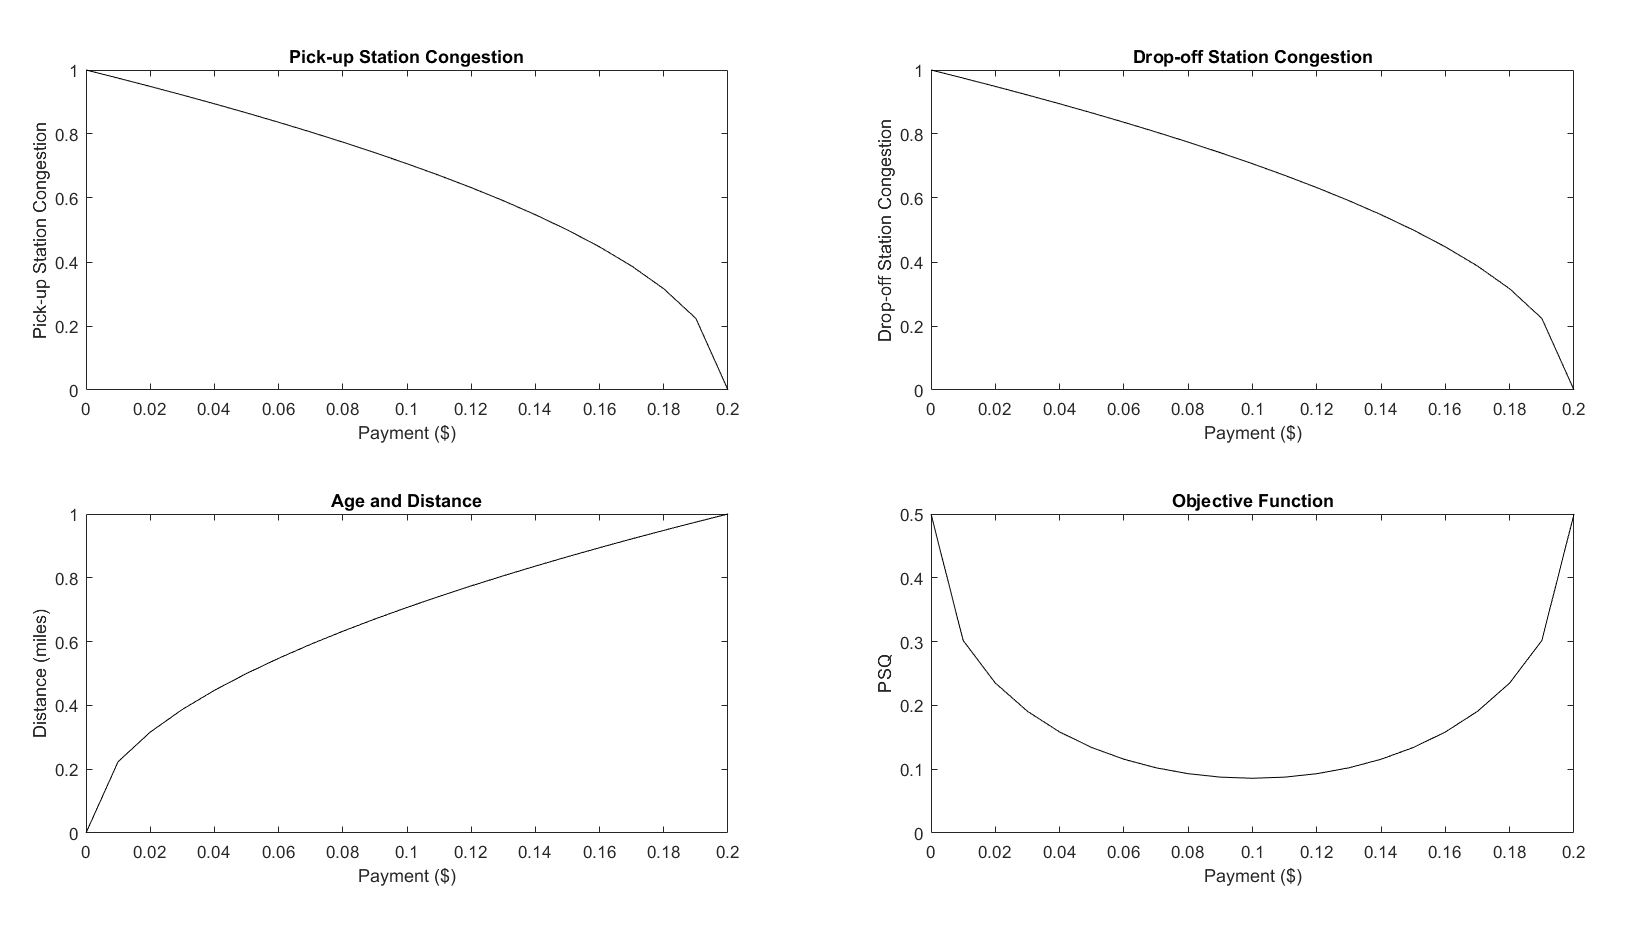
\includegraphics[width=0.5\textwidth]{m4/poster_plot.png}}
\centerline{Figure 1: Convex Optimization Example}
\hfill \break

%\subsection{Constraints}
%
%The objective function has a few constraints. First, the distance ($d_{puc}$ and $d_{duc}$) between each candidate station and a user's intended station must not exceed the maximum distance the user is willing to walk ($r_u$). Second, each station's capacity ($C_s$) cannot be exceeded by the station's number of current bikes ($v_s$). Third, the budget available to each user ($p_u$) in the network for time interval $t$ is constrained by the total budget ($B$) and the number of users in the system ($n$).
%
%\begin{equation}
%d_{puc} \leq r_u
%\end{equation}
%\begin{equation}
%d_{duc} \leq r_u
%\end{equation}
%\begin{equation}
%v_s \leq C_s
%\end{equation}
%\begin{equation}
%p_u \leq B/n
%\end{equation}
%\begin{equation}
%0 \leq \textnormal{all parameters except } D_u
%\end{equation}

%Lastly, the convex optimization problem is formulated in the form of an objective function with constraints. First, we define a few parameters: denote the m stations in the Citi Bike network by the set S = {s1, s2, ... sm}, the maximum bike docks by Cs and the number of bikes available at time t at station s by v(s,t). Assume that a user u with subscription type S and age A intends to pick up a bike from station s(u,1) and head towards station s(u,2). As an attempt to influence the user's decision, the incentive system will suggest two lists of alternative stations, s(*,1) and s(*,2), with associated monetary incentives p*. %p* belongs to P, where P = {pmin, p2, ..., pmax} is a set of fixed prices. A budget B is allocated for the system for a time itnerval t. Lastly, ru represents the maximum distance u is willing to walk.
%
%These parameters are then used to define a set of sub functions:
%% bullet points?
%Congestion: Using the difference between the station's in degree and out degree to estimate the expected number of open docks in the future, the congestion level of bike station s is expressed as 
%\centerline{Cg=Cs-v(s,t)+ks(out degree-in degree)}
%
%Alternative Stations: the lists of alternative stations are determined by ru and the distance between the user's intended station and other bike stations in the set S.
%\centerline{if dist(s(u,1,2), si|si belongs to S) <= ru}
%\centerline{si belongs to s(*,1,2)}
%
%Monetary Incentives: the payment for the user is modeled as a function of 
%
%User dissatisfaction: since the incentives system attempts to alternate the user's initial decision, 

%------------------------------------------------------------------------- 
\section{Experimental Setup and Practical Results}

\subsection{Network Analysis}
Based on the network definition presented at the beginning of Section 4, a sample dynamic network is constructed to represent bike usage from Thursday to Saturday in a normal week. First, Citi Bike data from the first three days of September 2016 is extracted from the original data set in \cite{dataset} to generate a node table with 583 nodes and an edge list with more than 130,000 edges. Second, the node table and edge list are imported to Gephi as a dynamic network. The Gephi plugin \textit{Geo Layout} is used to arrange the nodes according to their geographic locations, while network properties are dynamically changed by filtering out edges outside a particular time window. In this analysis, the time window for edge filtering is set to one hour.\\

\centerline{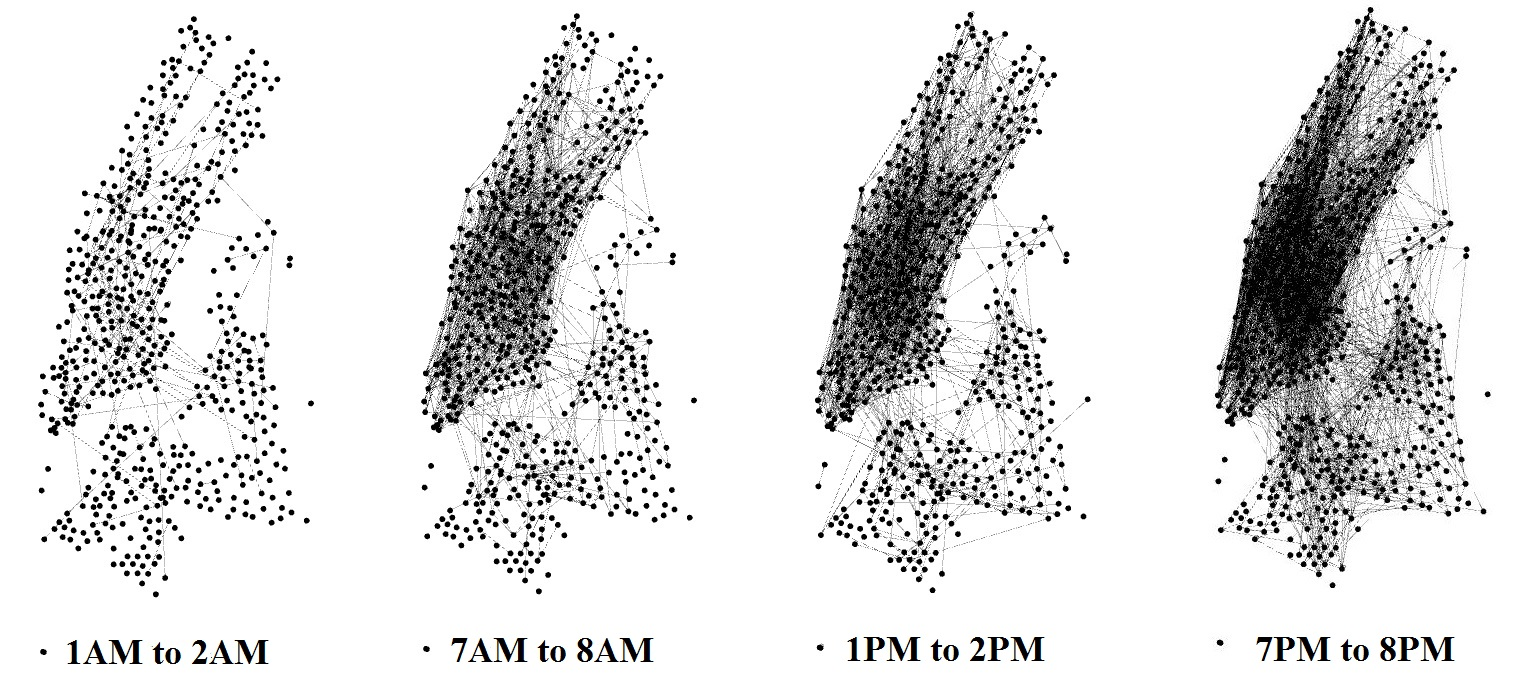
\includegraphics[width=0.5\textwidth]{m4/combined.jpg}}
\centerline{Figure 2: Citi Bike Network on September 1, 2016}
\hfill \break
\indent Figure 2 shows the network at four different time intervals on September 1, 2016. From left to right, the layouts represent the network between 1\textsc{am} and 2\textsc{am}, 7\textsc{am} and 8\textsc{am}, 1\textsc{pm} and 2\textsc{pm}, and 7\textsc{pm} and 8\textsc{pm}. Figure 3 illustrates how some of the network properties change over time. Every day, the maximum average node degree is observed between 4\textsc{pm} and 7\textsc{pm}, corresponding to the evening rush hour. On the two weekdays, there is also a secondary peak between 7\textsc{am} and 8\textsc{am}, reflecting the morning rush hour. As expected, this secondary peak is not present on September 3 since it is a Saturday. Unlike the average node degree, the network's average path length stays relatively consistent during the day and in the early evening. Bikers seem to take longer trips around midnight and in the morning (between 6\textsc{am} and 7\textsc{am}), while the trips between midnight and 6\textsc{am} tend to be much shorter.

\centerline{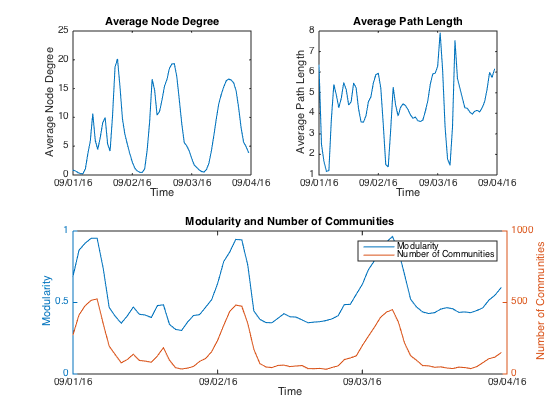
\includegraphics[width=0.5\textwidth]{m4/plotterfigure.png}}
\centerline{Figure 3: Citi Bike Network Properties}
\hfill \break
\indent As for community structure, the network's modularity and formation of communities exhibit a periodic pattern. During the day, the network has high modularity and the nodes can be grouped into a few communities. At night, the network is less modular and only a handful of nodes form communities with others. This observation is in line with the fact that bike movement patterns tend to be unidirectional during the day (when bikers go to work) and disperse at night (when bikers go home in different directions).

This network setup has a few limitations. One limitation is that the congestion level at each station (i.e. maximum capacity versus current number of stored bikes) is not taken into account. In addition, only a very small subset of the available data is exploited. These issues are addressed in Section 5.2 by simulating the network.

\subsection{Citi Bike Network Simulation}

In order to demonstrate whether or not the formulated optimization problem results in decongesting the Citi Bike network, a simulator is created using MATLAB. The simulator first uses an entire month's trip data plus data from the beginning of the next month to implement the initialization procedure and estimate how many bikes are at each station. Beginning with a specified date in the next month, trip data entries are stepped through for a time period specified by the user. Each entry has a start station and an end station corresponding to the biker's intended pick-up and drop-off stations ($s_{pu}$ and $s_{du}$).

If the congestion level is high for one or both of these intended stations (too empty for pick-up or too crowded for drop-off), the user is provided with a pair of alternative pick-up and drop-off stations ($s_{puc}$ and $s_{duc}$). This pair is determined deterministically to locally minimize congestion as explained in Section 4.3. The convex optimization problem then uses information about this alternative pair of stations to compute an associated payment for the user that minimizes PSQ subject to budget constraints. Lastly, a probability model is used to estimate whether or not the user accepts the payment and takes the alternative route.

\hfill \break
\centerline{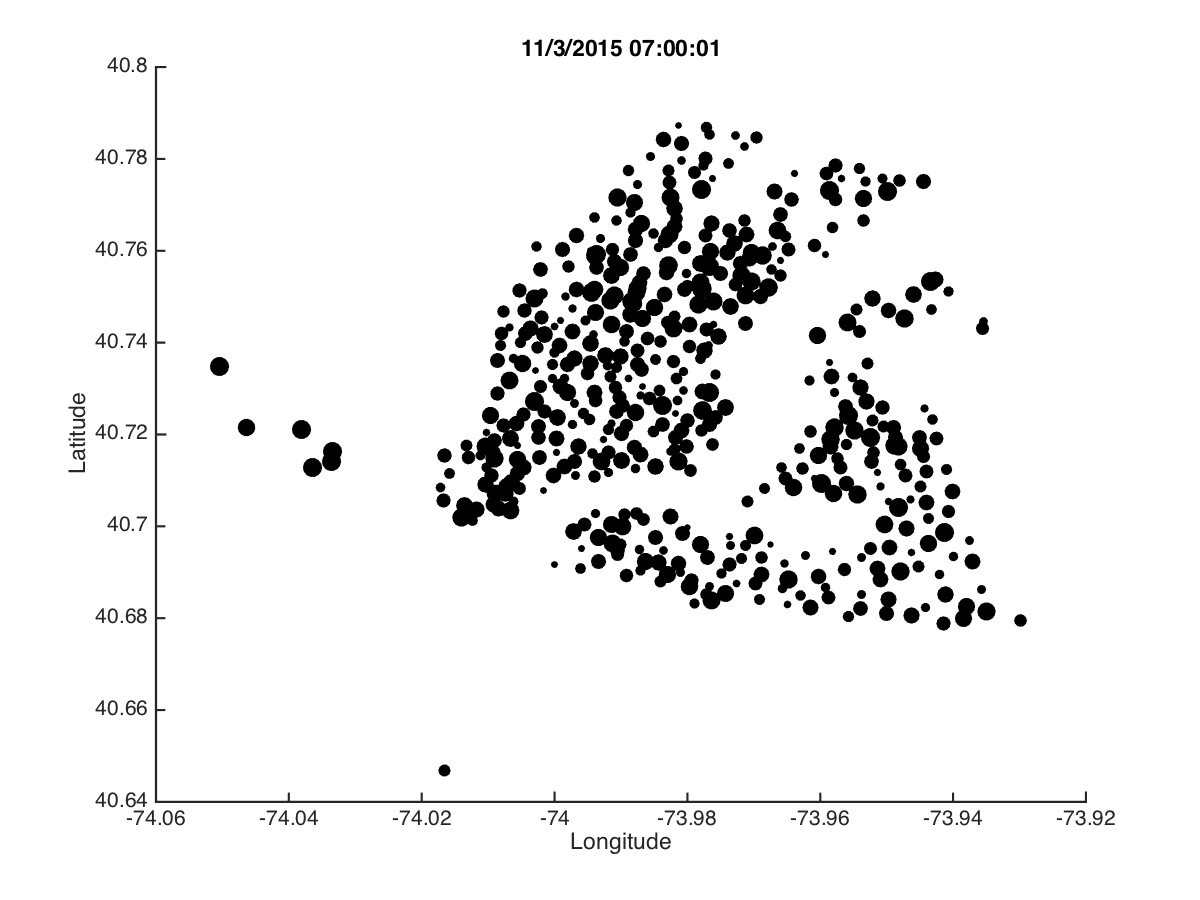
\includegraphics[width=0.25\textwidth]{m4/no_incentives_before.png}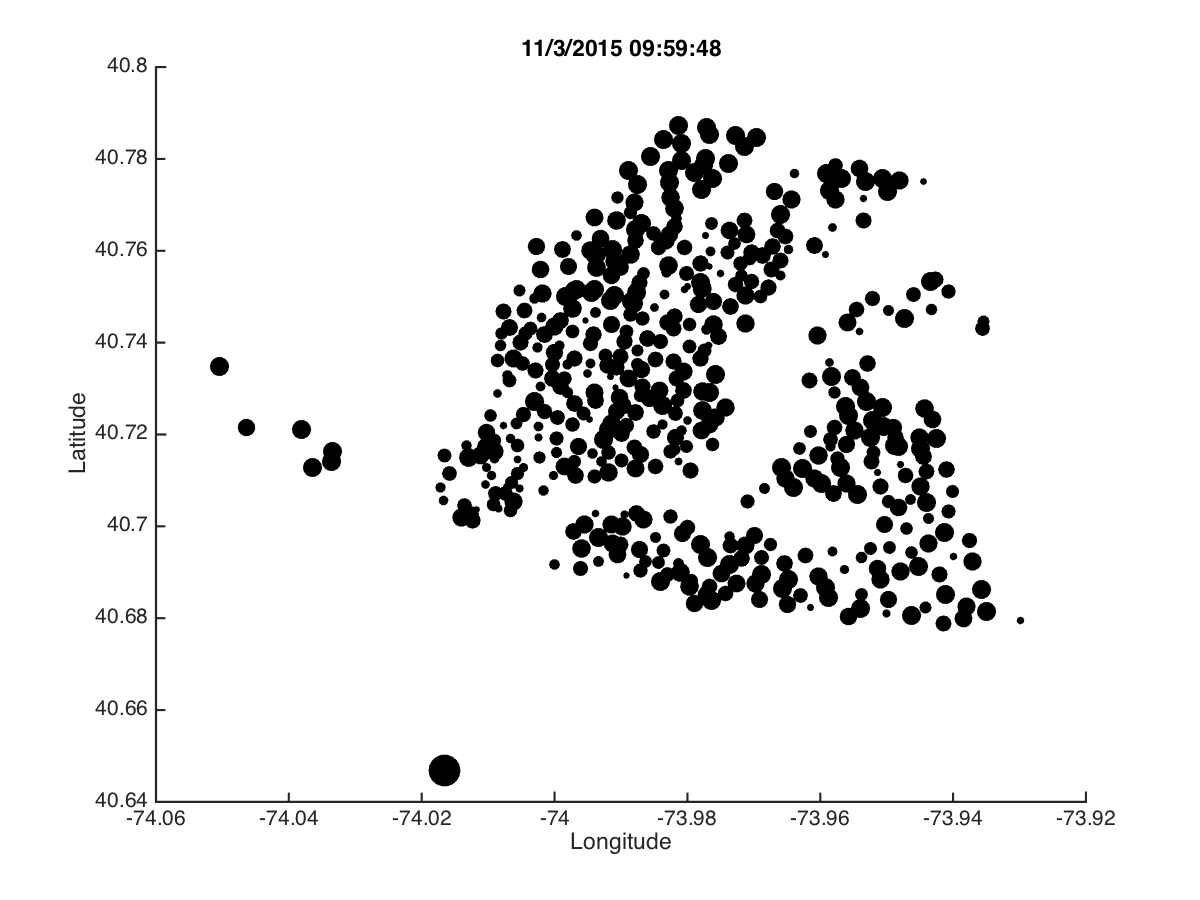
\includegraphics[width=0.25\textwidth]{m4/no_incentives_after.png}}
\centerline{Figure 4: Citi Bike Network with No Incentives}
\hfill \break
\centerline{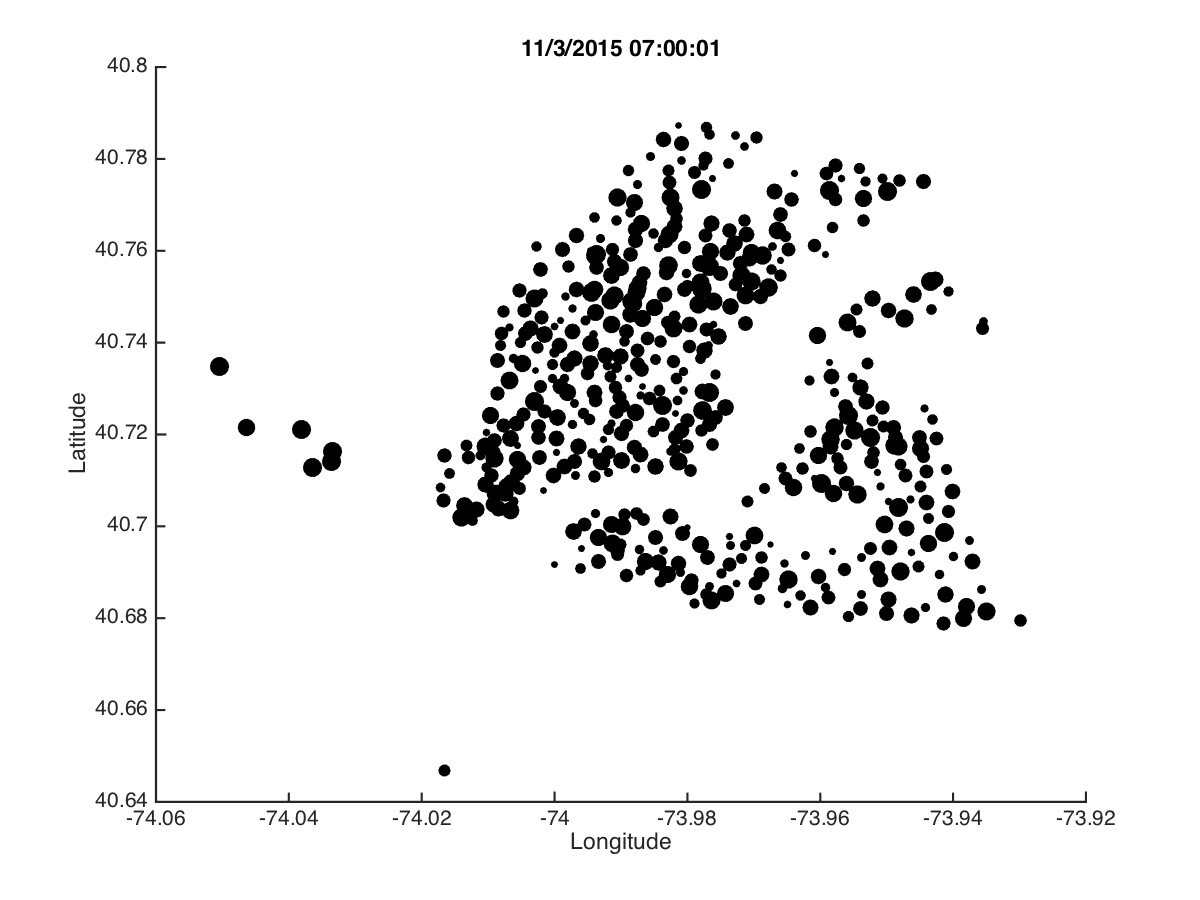
\includegraphics[width=0.25\textwidth]{m4/incentives_before.png}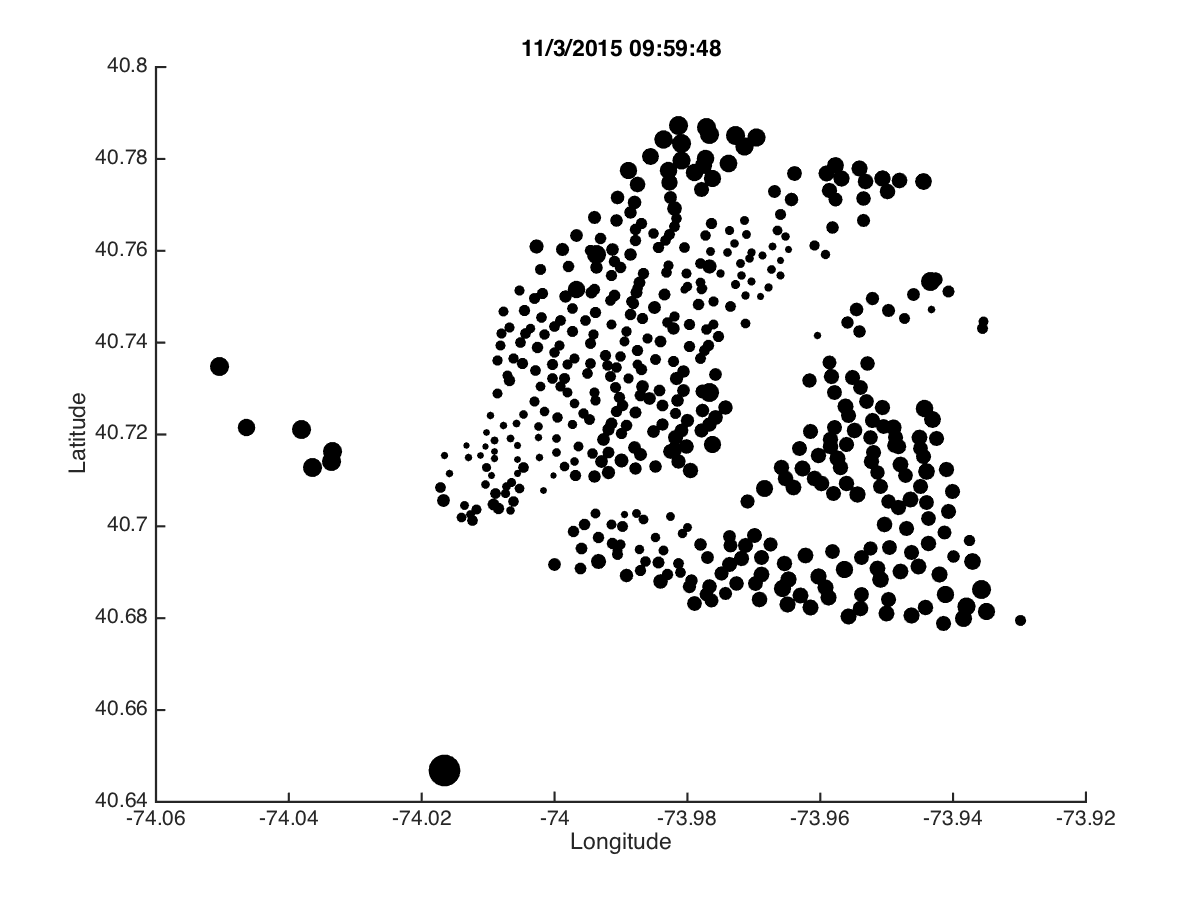
\includegraphics[width=0.25\textwidth]{m4/incentives_after.png}}
\centerline{Figure 5: Citi Bike Network with Incentives}
\hfill \break
\indent After the user makes a decision about the incentive, the state of the Citi Bike system is updated with respect to the number of bikes at each station. Figure 4 shows the state of the Citi Bike system at 7\textsc{am} and 10\textsc{am} on March 3, 2016 with no monetary incentives. Figure 5 shows the state of the system at the same times when bikers always choose to take the incentives. In each figure, the dots represent the bike stations, and the size of a dot is proportional to the deviation of currently stored bikes from half of the station's capacity. In other words, a large dot indicates that the bike station is either too empty or too full, thereby causing pick-up or drop-off congestion. As shown, the network stays relatively congested when bikers are not provided with any incentives, but the network quickly decongests itself when all bikers accept the monetary incentives. This result demonstrates that the properties of the network can be changed significantly if enough bikers accept the monetary incentives.

Although the simulator overcomes the limitations of the basic network setup described in Section 5.1, it has a few limitations of its own. First, there is no information about the maximum capacity for approximately 10\% of the bike stations, so an estimate must be used. Second, there is no data about bikes being moved to other stations by trucks, so this flow of bikes is unaccounted for. Because of this lack of information, the initialization procedure and simulation of the Citi Bike system is slightly inaccurate.

\subsection{Probability Model and System Performance}
Currently, two probability models are deployed to simulate a user's acceptance of monetary incentives. First, a linear model is used to directly correlate user acceptance with payment $p_u$. The probability of acceptance is 1 if the user is offered the maximum payment $B/n$, otherwise the probability decreases linearly with $p_u$. In other words, 
\begin{equation}
P = \frac{p_u}{B/n}
\end{equation}
Using this probability mode, we ran the network simulation on four different days and time intervals and calculated average PSQ and system congestion. The results are shown in Figure 5.

The second probability model is used to investigate what percentage of the population need to accept the monetary incentives in order to significantly decongest the system. We ran the network simulation on November 3, 2015 from 7am to 10am and varied the probability from 0 to 1 with a step size of 0.1. Figure 6 shows the average PSQ and system congestion with different probabilities. While average PSQ decreases proportionally with probability, average system congestion reduces aggressively as more bikers accept the monetary incentives. Eventually, average system congestion reaches saturation and having a larger percentage of the population accept the monetary incentives does not dramatically change the average system congestion. In fact, the results suggest that only half of the population need to accept the monetary incentives before average system congestion approaches its saturation level.

%\centerline{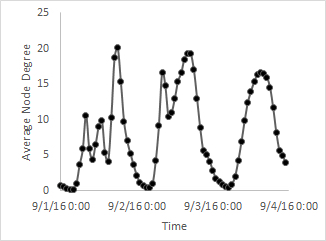
\includegraphics[width=0.4\textwidth]{node_degree.jpg}}
%\centerline{Figure 2: Average Node Degree}
%\vspace{5mm}

%\centerline{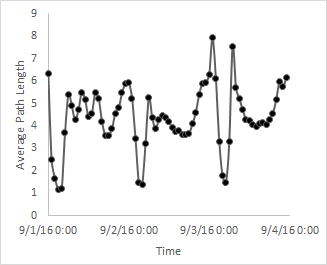
\includegraphics[width=0.4\textwidth]{path_length.jpg}}
%\centerline{Figure 3: Average Path Length}
%\vspace{5mm}

%\centerline{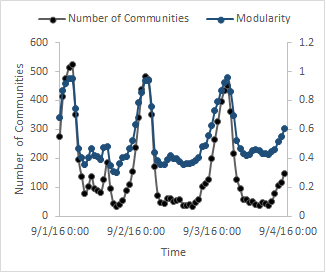
\includegraphics[width=0.4\textwidth]{communities.jpg}}
%\centerline{Figure 4: Modularity and Number of Communities}

%------------------------------------------------------------------------- 
\section{Conclusion}
This work proposes a network-based framework to decongest the Citi Bike system via convex optimization. After constructing the system as a dynamic network, the objective function, constraints, and other related functions and parameters are defined for the convex optimization problem. A thorough analysis of the Citi Bike network's properties is completed, and a MATLAB simulator is used to modify the network's properties using monetary incentives.

Future work may explore reducing congestion by altering the network topology through optimal placement of nodes (stations). Future work should also modify the monetary incentives acceptance probability model used in the simulation so that it depends on both payment and the distance a user has to walk. In addition, future work may explore modifying the maximum walking distance model to include both the user's age and the distance the user intends to travel. Future work should also analyze the effect of giving users a set of alternative station pairs as opposed to only one alternative station pair. Lastly, future work may conduct an in-depth analysis as to what the overall spending budget $B$ should be to best minimize congestion and still result in a profit for Citi Bike.

%the percentage of bikers needed to accept monetary incentives and cause a significant decrease in system congestion will be determined.
%The basic methodology to construct the Citi Bike network is proposed in this work. Because certain information is not available about the bike stations' capacity, an initialization procedure is also proposed to estimate the number of bikes in the system and at each station. As a preliminary analysis, a sample network is constructed using data between September 1, 2016 and September 3, 2016 to evaluate network properties at different time intervals. In this work, Paul Griffioen extracted network information from the original dataset using MATLAB and Anthony Jin analyzed the network using Gephi.

%The next step of this project is to overcome the limitations of the experimental setup and construct the complete Citi Bike network. By Milestone 2, we will finish the network analysis and begin implementing the pricing scheme.

%------------------------------------------------------------------------- 
%\Section{Overview}
%
%The Citi Bike system, located in New York City, is one of many bicycle sharing systems that exist in the world. Since users unlock a bike at one station and drop it off at another station, bikes tend to follow unidirectional flows at various times of the day. As a result, some stations have few to no bikes at them while others are completely full.
%
%This unidirectional flow of bikes frustrates users who would like to pick up a bike from an empty station or drop off a bike at a full station. As a result, this project seeks to address the bicycle congestion problem by introducing a congestion-based pricing scheme that modifies the incentives of users. It takes a unique approach by solving the congestion problem from a network standpoint as opposed to other viewpoints, such as that presented in \cite{incentives}.
%
%%------------------------------------------------------------------------- 
%\Section{Objectives and Deliverables}
%
%This project seeks to address the issue of system congestion through a pricing scheme based on the optimization of network structure and dynamics. In addition, alteration of the network topology to reduce congestion will be explored through optimal placement of nodes (stations). Large amounts of publicly available data from Citi Bike's website will be used as the main dataset for this project \cite{dataset}. The deliverables for this project include presenting progress, formulating a paper, and participating in a conference-style presentation. In the end, this project seeks to analyze the Citi Bike network and minimize congestion by modifying its structure through changing people's incentives.
%
%%------------------------------------------------------------------------- 
%\Section{Tasks and Timeline}
%
%To accomplish the objectives aforementioned, a timeline with associated tasks is proposed as follows.
%\textit{Network Formulation}: Two to three weeks should be used to build weighted networks of trips for each month using the data found in \cite{dataset}.
%\textit{Network Analysis}: About three weeks should be used to compare the weighted networks in the context of different factors such as weather and seasonality, the time of day, and the day of the week. Additionally, potential user incentives should be identified.
%\textit{Optimization Using Congestion-Based Pricing Scheme}: The congestion-based pricing scheme will take four to five weeks to develop and will deploy the identified user incentives. Specifically, the scheme will feature a user incentive model based on the mathematical models proposed in \cite{incentives} and \cite{redistribution}. In addition, a convex optimization problem will be formulated to account for related objective functions (i.e. minimizing congestion) and constraints (i.e., cost of operation) \cite{sharing} \cite{management}. Ultimately, this scheme aims to optimize the existing network by changing its weights and decreasing congestion.
%\textit{Optimization of Network Topology}: If time permits, an additional task is to examine the topology of the existing network and make appropriate changes to its physical structure by optimizing the placement of nodes.
%
%%------------------------------------------------------------------------- 
%\Section{Conclusion}
%
%This project aims to optimize the Citi Bike network via a congestion-based pricing scheme. Specifically, this scheme will change user incentives and will consequently modify the network's weights while minimizing congestion.

%------------------------------------------------------------------------- 
\nocite{ex1,ex2}
\bibliographystyle{paper}
\bibliography{paper}

%\begin{thebibliography}{}
\begin{thebibliography}{}\setlength{\itemsep}{-1ex}\small

\bibitem{incentives}
A. Singla, M. Santoni, G. Bartok, P. Mukerji, M. Meenen, and A. Krause. "Incentivizing Users for Balancing Bike Sharing Systems." \textit{AAAI}, pp. 723-729, 2015.

\bibitem{redistribution}
J. Pfrommer, J. Warrington, G. Schildbach, and M. Morari. "Dynamic Vehicle Redistribution and Online Price Incentives in Shared Mobility Systems." \textit{Intelligent Transportation Systems, IEEE Transactions on}, 15(4): 1567-1578, 2014.

\bibitem{sharing}
M. Rainer-Harbach, P. Papazek, B. Hu, and G. R. Raidl. "Balancing Bicycle Sharing Systems: A Variable Neighborhood Search Approach." \textit{Springer}, 2013.

\bibitem{management}
T. Raviv and O. Kolka. "Optimal Inventory Management of a Bike-Sharing Station." \textit{IIE Transactions}, 45(10): 1077-1093, 2013.

\bibitem{dataset}
Citi Bike, "System Data." Motivate International, Inc. Accessed 22 September 2016. [Online]. Available: https://www.citibikenyc.com/system-data.

\end{thebibliography}

\end{document}
